%
% Main thesis LaTeX file. We use the REPORT style format
% instead of article for most technical papers
%
%
\documentclass[11pt,fleqn]{article}

%%%%%%%%%%%%%%%%%%%%%%%%%%%%%%%%%%%%%%%%%%%%%%%%%%%%%%%%%%%%%%%%%%%%
%
% list the set of packages we use for various aspects of 
% the thesis format
%
\usepackage{layout}
\usepackage[utf8]{inputenc}
\usepackage{setspace}

\usepackage{tabularx}
\usepackage{subfigure}
\usepackage{epsfig}
\usepackage{float}
\usepackage{floatflt}
\usepackage{listings}
\usepackage{palatino}
\usepackage{verbatim}
\usepackage{footnpag}
\usepackage{caption}
\usepackage[mathcal, mathbf]{euler}
\usepackage{amsmath}
\usepackage{amstext}
\usepackage{color}
\usepackage{xcolor}
\usepackage{graphicx}


%%%%%%%%%%%%%%%%%%%%%%%%%%%%%%%%%%%%%%%%%%%%%%%%%%%%%%%%%%%%%%%%%%%%
%
% include two local LaTeX source files that establish the
% thesis layout and the set of additional commands we find
% useful for creating the text.
%
\input{layout}
\input{newcommands}
\input{outline_support}


\newcommand{\Organization}{School of Computer Engineering}

\title{CE2007 Lab Report}

\author{
  Lu Shengliang \\
  Group: SEP1 \\
  U1220521C \\
  \Organization{} \\
  \vspace*{-10mm} \\
  Nanyang Technological University \\
  \vspace*{-10mm} \\
  SLU001@e.ntu.edu.sg
}

%
% This begins the actual lab report
%
\renewcommand{\OutlineLevel}{2}

\begin{document}

\maketitle

\ls{1.2}


\section{Lab 1 - Assembly Language}

%=====================================================================
\subsection{$\mu$Vision4 Development tools configurations setup}
The configuration for Target is shown below.
\begin{enumerate}
  \item crystal speed Xtal = 50MHz
    This Xtal indicate our internal clock speed is 50MHz, which is the speed of our ARM processor.
  \item Internal Read/Only Memory Areas: Start address = 0x0 and Size = 0x8000
    Where we are setting is the address location of on-chip ROM, which is from 0x0 to 0x7FFF. We set it as startup location and we will load our code in this ROM.
  \item Internal Read/Write Memory Areas: Start address = 0x20000000 and Size = 0x4000
    Where we are setting is the address location of on-chip IRAM, which is from 0x20000000 to 0x20003FFF. Data Tightly-Coupled Memory or the memory our codes need are stored here.
\end{enumerate}
\begin{figure}[H]
\centering
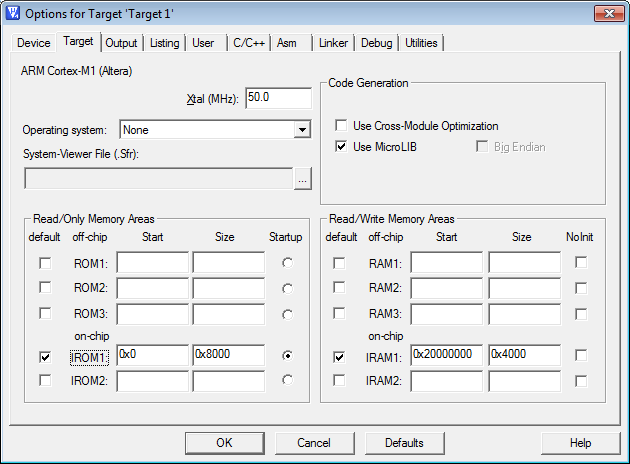
\includegraphics[width=\textwidth]{configuration.png}
\caption{Target configurations}
\end{figure}

Other settings are omitted here.

%=====================================================================
\subsection{Exercise A. Blink\underline{ }LED.s}
Let us have a look at the top several lines of this assembly code.
\lstset {
    language=[x86masm]Assembler,
    backgroundcolor=\color{black!5},
    basicstyle=\ttfamily\footnotesize,
    numbers=left,
    numberstyle=\tiny,
    frame=single
}
\renewcommand{\baselinestretch}{0.75}
\begin{lstlisting}
         AREA   STACK, NOINIT, READWRITE, ALIGN=4; Name block of code
                                                 ; as STACK, reside
                                                 ; in RAM area
  Stack_Size	EQU	0x200            ; Stack Size = 0x200 bytes
  Stack_Mem	SPACE	Stack_Size       ; Reserve the space in RAM
  TOP_STACK                              ; Set top of stack location
\end{lstlisting}
\end{\baselinestretch}
This piece of code indicates the stack size of startup. Stack is built up for runtime data allocation, which means that we should put stack to location to 0x20000000 to 0x200001FF. the TOP\underline{ }STACK will be at 0x20000200. \\
%=====================================================================

\renewcommand{\baselinestretch}{0.75}
\begin{lstlisting}
	AREA	RESET, DATA, READONLY
__Vectors	DCD	TOP_STACK	; Vector table start here
                                        ; first entry is Top of stack
		DCD	START		; second entry is the Reset
\end{lstlisting}
\end{\baselinestretch}
This piece of code initialize the vector table. Firstly, vector table should be read-only, which indicates its location will be ROM area. Of course, the first entry of vector table should contain the location of TOP\underline{ }STACK location. It will be used to initialize Main Stack Pointer(MSP) value by putting the first entry value into it.
Then we set second entry Reset vector using "DCD START", which determines the program execution starting address. The data in reset vector will be loaded into program counter, PC.
\renewcommand{\baselinestretch}{0.75}
\begin{lstlisting}
	AREA	texts, CODE, READONLY
ENTR				; Mark first instruction to execute
START		PROC		; Declaration of subroutine/function
\end{lstlisting}
\end{\baselinestretch}
As we can see here, user application codes should be put into ROM area. And the constant START is assigned here.
\renewcommand{\baselinestretch}{0.75}
\begin{lstlisting}
		MOVS	R2,#0xA
		LSLS	R2,R2,#28
leds_on		MOVS	R0,#0xFF        ; To turn on all 10 LEDs
                                        ; value need = 0x3FF;   
                LSLS	R0,R0,#2
\end{lstlisting}
\end{\baselinestretch}
The first 2 lines of this piece of code is just setting R2 as 0xA000000, which is the address of LEDs on DE0 board. Later we can just \textbf{\emph{STR}} the binary value to enable lights accordingly. \\
Before we put desired value into the memory entry, we must set the value in to a register. Here is the error of the code occurred. Instead of putting 0xF5, we should put 0xFF here like the code shows above.
\subsection{Understanding .map file}
\begin{figure}[H]
\centering
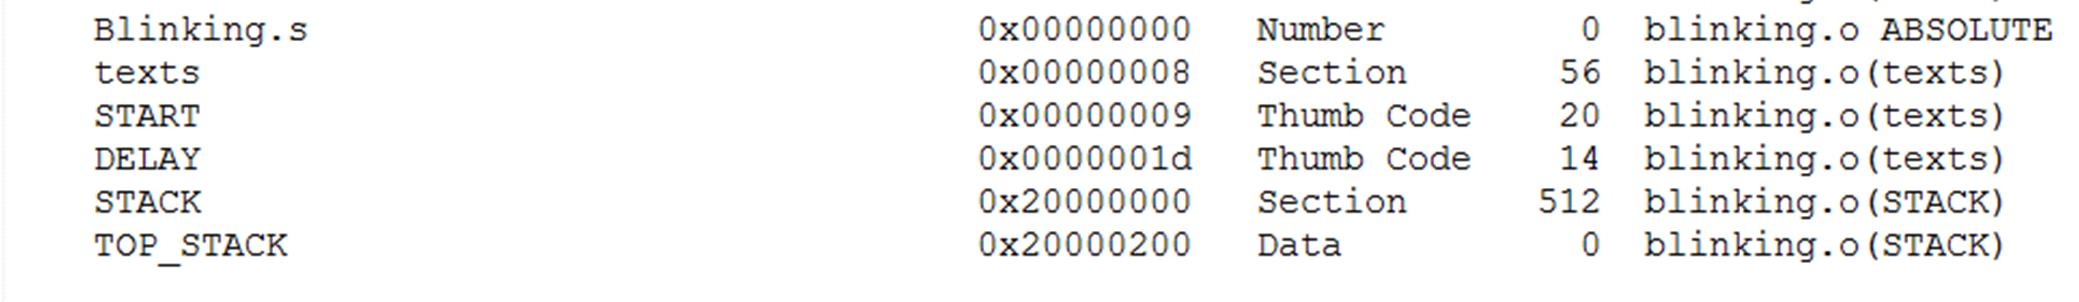
\includegraphics[width=\textwidth]{dotMapFile2.png}
\caption{.map file}
\end{figure}
The configurations of assembly code are already discussed above. This .map file gives the details about each parameter we set.\\
For example, \textbf{\emph{START}} indicates the program is stored with the start entry as 0x00000011.
\subsection{Exercise B. Blink\underline{ }LED.s in an alternate pattern}
In order to blink the \textbf{\emph{odd}} and \textbf{\emph{even}} LEDs in an alternate pattern, what we should do is to light odd or even LEDs first and then turn off them, turn on the others.

\renewcommand{\baselinestretch}{0.75}
\begin{lstlisting}
odd_leds_on	MOVS	R0,#0xAA           ; R0 0010101010
		LSLS	R0,R0,#2           ; R0 1010101000
		ADDS	R0,#0x02           ; R0 1010101010
		STR	R0,[R2,#0x00]      ; put into LEDs
		BL	DELAY
even_leds_on	MOVS	R0,#0x55           ; R0 0001010101
		LSLS	R0,R0,#2           ; R0 0101010100
		ADDS	R0,#0x01           ; R0 0101010101
		STR	r0,[r2,#0x00]      ; put into LEDs
		BL	DELAY
		B	leds_on            ; jump back, repeat
\end{lstlisting}
\end{\baselinestretch}

\subsection{Exercise C. Blink\underline{ }LED.s in an alternate pattern}
First of all, the code below shows the way to get the address of slide switches.
\renewcommand{\baselinestretch}{0.75}
\begin{lstlisting}
MOVS	R5,#0xA            ; put R5 as 0x0000000A
LSLS	R5,R5,#16          ; shift R5  0x0000A000
ADDS	R5,#0x01           ; append 1  0x0000A001
LSLS	R5,R5,#12          ; shift R5  0xA0001000
\end{lstlisting}
\end{\baselinestretch}
Now, in order to get the value of slide switches, at the start of each loop, we should access data contain at R5.
\renewcommand{\baselinestretch}{0.75}
\begin{lstlisting}
leds_on		LDR	R6,[R5]
\end{lstlisting}
\end{\baselinestretch}
The left work is just put R6 to the entry addressed by R2.
\renewcommand{\baselinestretch}{0.75}
\begin{lstlisting}
display	STRH	R6,[R2] ; Store the value to the DE0_LED address
	B	leds_on	; Repeat
\end{lstlisting}
\end{\baselinestretch}

%=====================================================================

\subsection{Exercise D \& E. 7-Segment display}
There are four 7-segment LEDs on the DE0, which are memory mapped to address at 0xA0004000. So in order to light these LEDs to display desired value, we can just load binary values into the address entry at 0xA0004000.

\renewcommand{\baselinestretch}{0.75}
\begin{lstlisting}
MOVS	R0,#0x01          ; 1
MOVS	R1,#0x06          ; 7-segment display of 1
SUBS	R0,R6,R0          ; compare R0 and slide switch
BEQ	display

MOVS	R0,#0x02          ; 2
MOVS	R1,#0x5B          ; 7-segment display of 2
SUBS	R0,R6,R0          ; compare R0 and slide switch
BEQ	display
\end{lstlisting}
\end{\baselinestretch}
After we loaded R6 with the switch value, we first load 1 into R0, load the display code into R1. We compare between R0 and slide switch. If they equal to each other, then we jump to display subroutine. The value of R0 will be loaded into 0xA0004000. \\
%====================================
\section{Lab 2 - C programming}

\subsection{Analyze startup.s}

\renewcommand{\baselinestretch}{0.75}
\begin{lstlisting}
Stack_Size  EQU     0x00000200
            AREA    STACK, NOINIT, READWRITE, ALIGN=3
Stack_Mem   SPACE   Stack_Size
__initial_sp
Heap_Size   EQU     0x00000400
            AREA    HEAP, NOINIT, READWRITE, ALIGN=3
__heap_base
Heap_Mem    SPACE   Heap_Size
__heap_limit
            PRESERVE8
            THUMB
\end{lstlisting}
\end{\baselinestretch}
The first part of the \emph{startup.s} is setting stack\underline{ }size as 0x00000200; the second part sets heap\underline{ }size to 0x00000400. Both of these area are available for read and write. \\
The last 2 lines of this piece of code indicate that our assembler will use THUMB IS, and the "PRESERVE8" directive specifies that the current code preserves 8-byte alignment of the stack/heap. We can refer to the setting of Stack/Heap, ALIGN=3. This argument tells that each instruction is aligned to 3 bytes. \\
The setting for vector table are similar to the previous lab. The differences are now we put Reset\underline{ }Handler instead of just START constant; and we put several handler, like NMI handler and Hard fault handler in the vector table following reset vector. \\



\subsection{Exercise A \& B. Blink\underline{ }LED.c}

\lstset {
    language=C,
    backgroundcolor=\color{black!5},
    basicstyle=\ttfamily\footnotesize,
    numbers=left,
    numberstyle=\tiny,
    frame=single
}
\renewcommand{\baselinestretch}{0.75}
\begin{lstlisting}
#define DE0_LEDs *((uint32_t *)(0xA0000000))

while (1) {
  DE0_LEDs=0x3FF; for (i=0;i<0x1FFFFF;i++); // on all LEDs & delay	
  DE0_LEDs=0x000; for (i=0;i<0x1FFFFF;i++); // off all LEDs & delay
}
\end{lstlisting}
\end{\baselinestretch}
The first line of this code define a pointer, which is the entry of address 0xA0000000. (uint32\underline{ }t *)(0xA0000000) casts an hexadecimal number to pointer of uint32\underline{ }t. Then the outside "*" makes DE0\underline{ }LEDs an memory entry, addressed by 0xA000000. \\
An infinity while loop stays in main function. The loop loads 0x001111111111 int DE0\underline{ }LEDs and then delay. After that, the code cleans LEDs into 0 and delay for the same period. \\
The length of time interval will depend on the limit of for loop and board internal clock speed. \\
Similarly, if we want to get the value of slide switches, we use the same method to get the contains of the entry.
In order to keep the corresponding LED following the slide switch, we can use \emph{OR} operation.
\renewcommand{\baselinestretch}{0.75}
\begin{lstlisting}
#define DE0_SLIDE_SW *((volatile uint32_t *)(0xA0001000))
DE0_LEDs = 0x2AA | DE0_SLIDE_SW;  //odd LEDs & slide switch
DE0_LEDs=0x155 | DE0_SLIDE_SW;    //even LEDs & slide switch
\end{lstlisting}
\end{\baselinestretch}
\subsection{Compiler Optimization Code}
\renewcommand{\baselinestretch}{0.75}
\begin{lstlisting}
#define DE0_SLIDE_SW *((uint32_t *)(0xA0001000))
\end{lstlisting}
\end{\baselinestretch}
Without declaring \textbf{\emph{volatile}}, the code works well with optimization level set to \emph{Level 0}, but not with configuration as \emph{Level 1}. The reason is: the development tool tends to optimize assembly code instead of just translating line by line. It notices that the code always loads from one memory address, which will be very slow. So the optimized way of loading from memory entry is make a copy of the memory entry stored in register. So our code will get value from register, which will be totally different from the DEO\underline{ }SLIDE\underline{ }SW when we trigger some switches. \\
But if we declare \textbf{\emph{volatile}}, development tool will take this as a changeable input, and will not make the code not working as what we expect.
\subsection{Exercise C. 7-segment display}
We address 7-segment LEDs with
\renewcommand{\baselinestretch}{0.75}
\begin{lstlisting}
#define DE0_7SEG_DISP *((volatile uint32_t *)(0xA0004000))
\end{lstlisting}
\end{\baselinestretch}
The rest of code are all arithmetic operations:
\renewcommand{\baselinestretch}{0.75}
\begin{lstlisting}
x = DE0_SLIDE_SW & 0x03;         // bit 0 and 1 of slide switch
y = (DE0_SLIDE_SW & 0x0C) >> 2;  // bit 2 and 3 of slide switch 
DE0_7SEG_DISP = (sevenSegCode[x + y] //sum put to first display
               + (sevenSegCode[x]<<16)
               + (sevenSegCode[y]<<24);
\end{lstlisting}
\end{\baselinestretch}
First, we get x as the last 2 bits of DE0\underline{ }SLIDE\underline{ }SW, y as the least 4th and 3rd bits. because x and y are both 2-bit, the sum of x and y will not exceed 6. we can use \emph{sevenSegCode[x + y]} directly to get the display code for the sum. \\
There are 4 7-segment display LEDs on DE0. So we just shift x's display code to bit 15 to bit 8, and shift y's display code to 23 to 16. So that 3 numbers will display on the board.
\subsection{Exercise D. ToneGen.c}
This exercise generates a digital number and loads it into an on-board \textbf{\emph{DAC}}, which direct the analog wave to a speaker.
\renewcommand{\baselinestretch}{0.75}
\begin{lstlisting}
for (countUp = 0; countUp < 16; countUp++){
  DAC_A = countUp; for(i = 0; i < 200; i++);
} //go up
for (countUp = 15; countUp >= 0; countUp--){
  DAC_A = countUp; for(i = 0; i < 200; i++);
} //go down
\end{lstlisting}
\end{\baselinestretch}
The code above generate a \emph{"triangular"} waveform, which has the same frequency as the given code. \\
The frequency generated by code depends on the \emph{"holding time"}. The original code has 16 values of each signal component, each of the value holds 400 counting time. The code showed above have 2 $\times$ 16 = 32 values of each signal component, and each of the value holds 200 counting time. So the total time interval is the same, which means the frequencies are the same. \\
If we decrease the holding cycles, the signal will become acuter than previous signal. It is because the frequency increasing leads the tone to rise. \\
It's also not difficult to make another shape of wave. like \emph{rectangular} wave:
\renewcommand{\baselinestretch}{0.75}
\begin{lstlisting}
for (countUp = 0; countUp < 16; countUp++){
  DAC_A = 15; for(i = 0; i < 400; i++);
}
for (countUp = 0; countUp < 16; countUp++){
  DAC_A = 0;  for(i = 0; i < 400; i++);
}
\end{lstlisting}
\end{\baselinestretch}
Instead of using the value of counter, we keep the DAC\underline{ }A as a constant. 15 is the upper edge of rectangular wave, and 0 is the lower edge. The sounds quite similar to triangular wave, except a bit strong that it. \\
One more thing should be noticed: the value of DAC\underline{ }A determines the loudness/volume of the sound. If we use 50 instead of 15, the sound will be much loader than previous one. The speaker came out with some rumble with DAC\underline{ }A = 50. \\

%=================================================================
\section{Lab 3: I/O interface through I$^{2}$C Bus}
\subsection{Introduction of I$^{2}$C Bus}
The introduction of I$^{2}$C is very sufficient on lab manual and lecture notes. The most important part of using I$^{2}$C bus is understanding the transfer sequence, which is defined by the relative timing transition \& states of the \textbf{\emph{SDA}} and \textbf{\emph{SCL}}. Details will be explained later.
\subsection{Exercise A. main3A.c}
Firstly, as usual, we need to study the code.
\renewcommand{\baselinestretch}{0.75}
\begin{lstlisting}
#define I2C_7SEG_Slave_Addr 0x40
write_with_start(I2C_7SEG_Slave_Addr);
write_with_stop(code[countUp]);
\end{lstlisting}
\end{\baselinestretch}
So how do we find the value of I2C\underline{ }7SEG\underline{ }Slave\underline{ }Addr?
\begin{figure}[H]
\centering
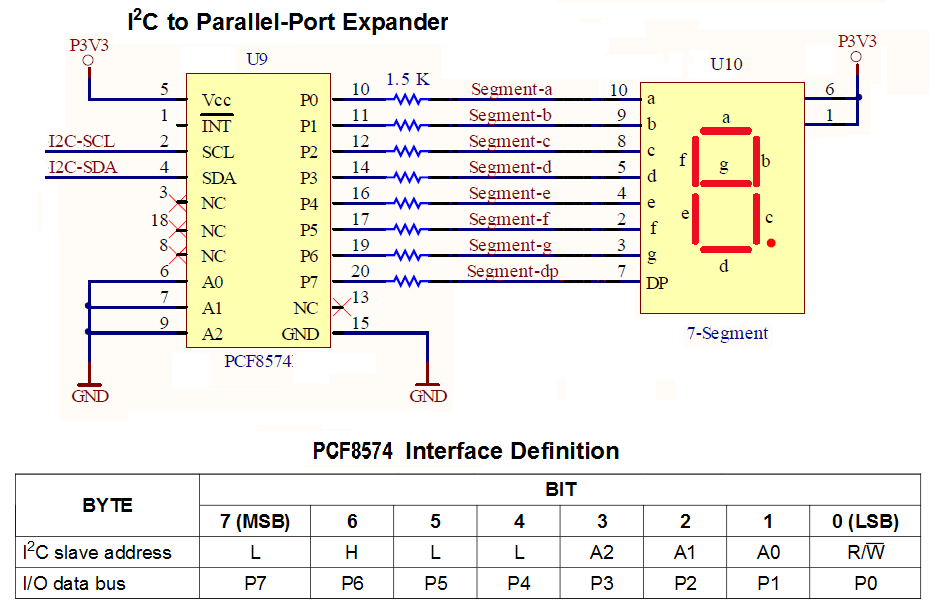
\includegraphics[width=\textwidth]{i2c_1.png}
\caption{Circuit Diagram \& Interface Definition}
\end{figure}
From the figure above we can see that I$^{2}$C slave address should be: Low, High, Low, Low, A2, A1, A0, R/W$^{*}$.
\begin{enumerate}
  \item R/W$^{*}$ should be 0, because we \emph{write} 7-segment code into display.
  \item A2, A1, A0 should be 0. From the circuit diagram we should know it, because pin A2, A1, A0 are connecting to \textbf{GND}.
\end{enumerate}
So, the I2C\underline{ }7SEG\underline{ }Slave\underline{ }Addr should be 0100 0000, which is 0x40.
The following main function consists of an infinity while loop; a count-up counter from 0 to 9; and a delay for loop after the two lines code shown above. \\
The first line shown above is the write\underline{ }with\underline{ }start(slave\underline{ }address). This function is declared in the header file \emph{i2c.h} and implemented in \emph{i2c.c}.
\subsubsection{Understanding write\underline{ }with\underline{ }start() function}
\renewcommand{\baselinestretch}{0.75}
\begin{lstlisting}
void write_with_start(uint8_t slave_add) {
  PUT_UINT8(I2C_BASE + TX_OFFSET, slave_add & 0xFE);
  // Writes slave address	
  PUT_UINT8(I2C_BASE + COMMAND_OFFSET, I2C_START | I2C_WRITE );
  // Sets control register bits	
  wait_for_eot();
  if (checkACK()) DE0_7SEG_DISP = ERRORCODE;
}
// #define TX_OFFSET    6   #define COMMAND_OFFSET     8
// #define I2C_BASE     0xA0008000
// #define I2C_START (1<<7) #define I2C_WRITE (1<<4)
// #define PUT_UINT8(address,  data)
\end{lstlisting}
\end{\baselinestretch}
Firstly, we use PUT\underline{ }UINT8 function, which is defined in \emph{main3.h}, to load first argument with the value of second argument. The first argument is an address. And second one is the data we want to load. We would like to load \textbf{\emph{Transmit register (TXR)}} with I$^{2}$C slave address. So, the first argument is I$^{2}$C base address $+$ the offset of \textbf{\emph{TX}} register. \\
Please be noticed that instead of using the slave address directly, the code uses \textbf{\emph{AND}} operation. This operation guarantees the last bit of data is 0, which is W$^{*}$ enable. \\
Secondly, we load \textbf{\emph{start}} and \textbf{\emph{write}} enable command into command register. \\
Next, we wait for end of transfer(eot) status, which is a function query from \textbf{\emph{Status register}} using polling check. It will stuck the bus until the bus is free. \\
Lastly, this function will check the \textbf{\emph{ACK}} from the recipient of data. \\
The other functional interfaces like write\underline{ }with\underline{ }stop are all similar to this.
\subsubsection{Understanding I$^{2}$C Transfer Sequence Diagram}
Here is a photo I took, when the I$^{2}$C bus is transferring number 4, whose 7-segment code is 0x99, to the LED display.\\
Firstly, on the top of oscilloscope screen, the green wave is clock, \textbf{\emph{SCL}}. It has 18 pulses, which means I$^{2}$C is transferring 2 bytes data, since 1 one extra clock for \textbf{\emph{ACK}} is appended to each byte. \\
The yellow wave on the bottom of the screen is the data wave of these 18 bits. 
\begin{enumerate}
  \item From the first positive edge to the first light blue line is the first byte.
    \begin{enumerate}
      \item Transfer starts with a go-down edge of \textbf{\emph{SCL}}, followed by go-down edge of \textbf{\emph{SDA}}.
      \item This byte indicates the slave address which is 0x40, 01000000.
    \end{enumerate}
  \item From the first light blue line to the green arrow mark is the second byte.
    \begin{enumerate}
      \item This byte is 0x99, the wave between two blue line indicate a 9, 1001.
      \item The rest indicates another 1001 followed by a clock cycle for \textbf{\emph{ACK}}.
    \end{enumerate}
  \item The green arrow shows that the small pulse is the stop signal.
    \begin{enumerate}
      \item Stop bit is a rising edge of \textbf{\emph{SDA}} followed by the rising edge of \textbf{\emph{SCL}}.
      \item The \textbf{\emph{SDA}} is low before the stop bit. In order to have a rising edge,  I$^{2}$C makes a pulse.
    \end{enumerate}
\end{enumerate}
\begin{figure}[H]
\centering
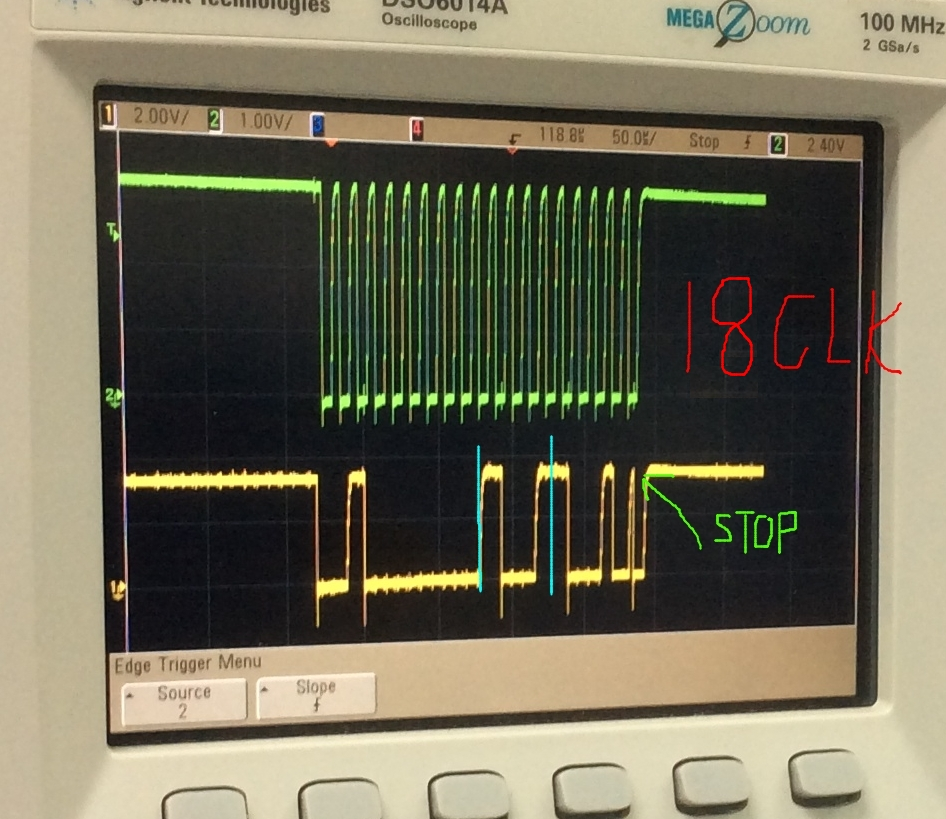
\includegraphics[width=\textwidth]{I2C_passing99.JPG}
\caption{I$^{2}$C transferring number 4}
\end{figure}
\subsection{Exercise B. Temperature Register}
\subsubsection{Obtain Slave Address}
The slave address should be easy to get from circuit diagram and slave addresses table with address pins.
ADD0 and ADD1 are connected to \underline{\textbf{GND}}. So they are both 0. After checking the table on the right, we can know slave address is 1001 0000, 0x90.
\begin{figure}[H]
\centering
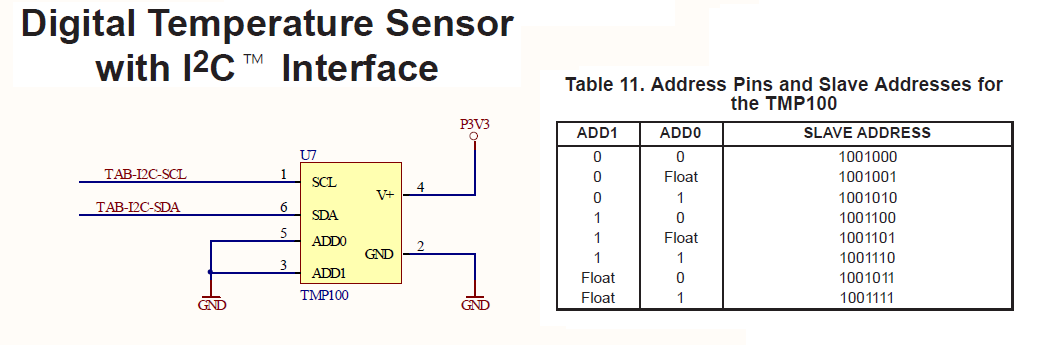
\includegraphics[width=\textwidth]{tmp100.png}
\caption{TMP100}
\end{figure}
\subsubsection{Access TMP100}
In order to access \emph{Configuration Reg} and \emph{Temperature Reg}, first thing we have to do is setting \textbf{\emph{Pointer Reg}} with desired register representative.
\renewcommand{\baselinestretch}{0.75}
\begin{lstlisting}
write_with_start(I2C_TEMP_SENSE_Slave_Addr);
write_byte(I2C_TEMP_SENSE_Conf_Reg);
write_with_stop(I2C_TEMP_SENSE_12bitRes);
\end{lstlisting}
\end{\baselinestretch}
So here what we are doing is accessing \textbf{\emph{Pointer Reg}} via I$^{2}$C, and write Conf\underline{ }Reg number/offset followed by the 12-bit resolution configuration in value. \\
We can only read the \emph{Temperature Reg} using the same strategy.
\renewcommand{\baselinestretch}{0.75}
\begin{lstlisting}
write_with_start(I2C_TEMP_SENSE_Slave_Addr);
write_with_stop(I2C_TEMP_SENSE_Temp_Reg);
read_with_start(I2C_TEMP_SENSE_Slave_Addr);
t1 = read_byte(); t2 = read_with_stop();
\end{lstlisting}
\end{\baselinestretch}
First, access \textbf{\emph{TMP100}} by sending slave address. Secondly provide \emph{Temperature Reg} representative. And then we can start reading from I$^{2}$C bus.
\subsubsection{Display in Celsius Format}
\renewcommand{\baselinestretch}{0.75}
\begin{lstlisting}
int tt;
tt = t1; //tt is in decimal
temp2 = t1 % 10;
temp1 = (t1 / 10) % 10;

temp3 = ((t2>>4) * 10 / 16); //Fractional part

temp1 =convertDigit(temp1);
temp2 =convertDigit(temp2);
temp3 =convertDigit(temp3);

temp1 = temp1<<16; temp2 = temp2<<8;
data = temp1|temp2|temp3;
\end{lstlisting}
\end{\baselinestretch}
As the code shows, we adapt \emph{uint8\underline{ }t} t1 to \emph{int} tt. Then put fractional part to temp3 by transferring the first 4 bits hexadecimal value to decimal. The original operation should be $HEX \times 16^{-1}$, which is fractional. In order to display it on 7-Segment LEDs, we $\times$ 10 to obtain the first digit after the decimal point. \\
Temp2 and temp1 stores the integer part. \\
We convert this digit to their corresponding display code, shift the code and merge to data. Data is the value we should load into 7-Segment LEDs address entry.
%=====================================================================
\end{document}
